% Interest of the model
Comme mentionné précédemment, à cause de la complexité du système il est préférable pour cette étude de considérer un sytème modèle.

% Description
    \subsection{Description du modèle}

Le système modèle est composé d'électrodes en graphites immergées dans un électrolyte aqueux d'hydroxyde de sodium, et sa structure est présentée à la \autoref{fig:schema_structure}.

\begin{figure}[htp]
    \centering
    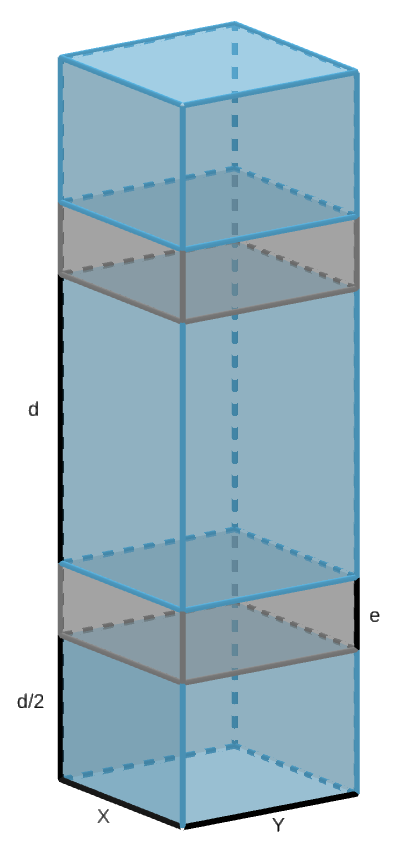
\includegraphics[height = 7cm]{schema_structure.png}
    \caption{Schéma de la structure du système modèle}
    \label{fig:schema_structure}
\end{figure}

Ses dimensions finales sont de \qtylist[list-units = single]{22.104;21.270;39.392}{\angstrom}, et les électrodes sont séparées d'environ \qty{20}{\angstrom} entre elles directement et à travers les conditions périodiques selon l'axe $[OZ)$.\\
Chaque électrode comprend \num{540} atomes de carbone. Après calcul, le nombre des molécules d'eau s'élèvent à \num{314}. Quant aux ions de l'électrolyte, nous avons choisi d'en introduire une dizaine de chaque pour pouvoir observer leurs déplacements.\\
Ainsi, le nombre total de particules dans le système s'élève à \num{2984}.

% Construction
    \subsection{Construction du modèle}

Pour construire la structure du modèle, la démarche \autoref{fig:construction_structure} a été adoptée.

\begin{figure}[hbp]
    \centering
    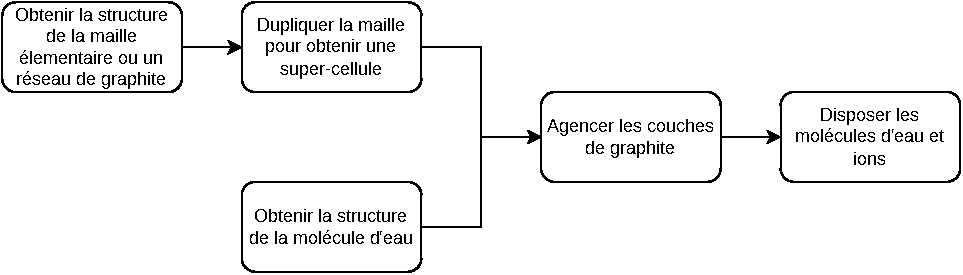
\includegraphics[width = \textwidth]{construction_structure.pdf}
    \caption{Démarche de construction de la structure}
    \label{fig:construction_structure}
\end{figure}

Tout d'abord, les données sur les structures des molécules ont été obtenues grâce à la \href{http://www.crystallography.net/cod/}{Crystallography Open Database} (COD) et celles-ci sont présentées à la \autoref{fig:molecules_initiales}.

\begin{figure}[hbt]
	\centering
	\begin{subfigure}[t]{.49\textwidth}
		\centering
		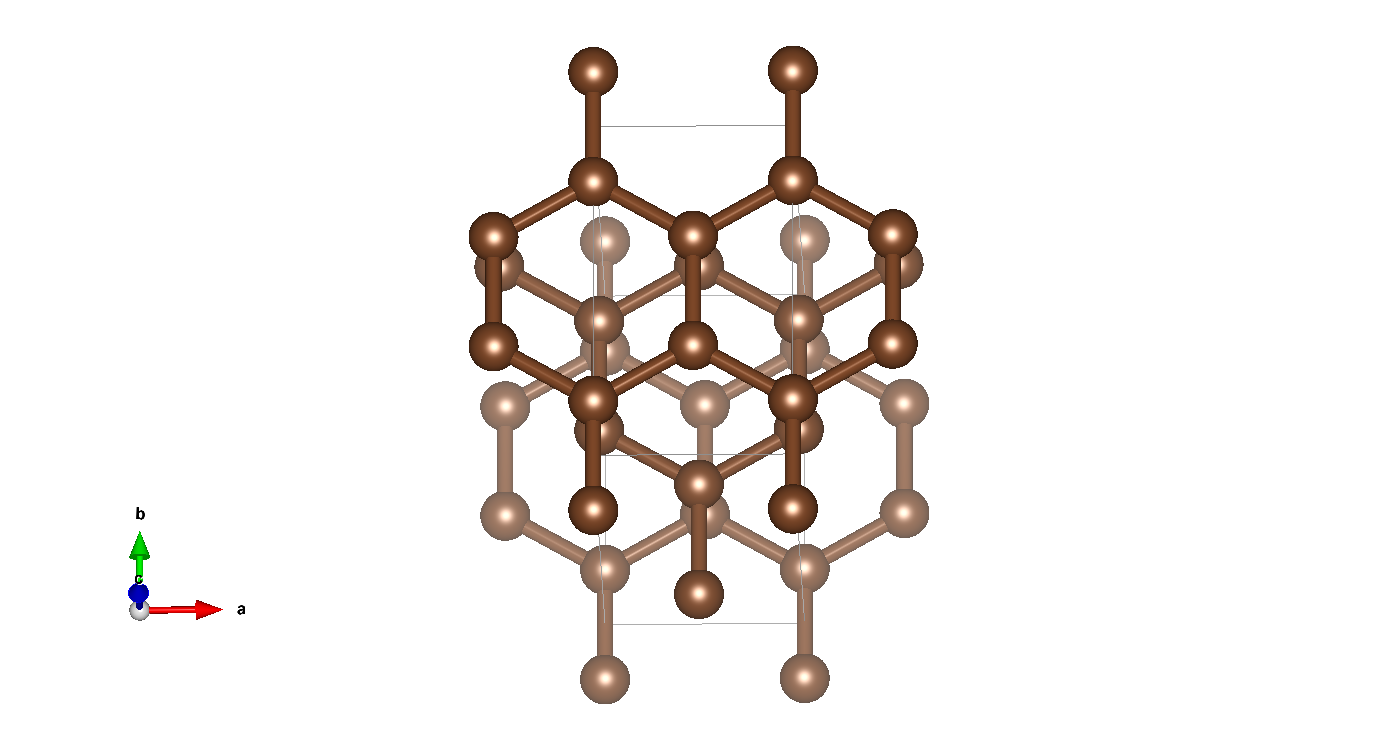
\includegraphics[width = \textwidth]{graphite.png}
		\caption{Réseau de graphite}
	\end{subfigure}%
    ~
	\begin{subfigure}[t]{.49\textwidth}
		\centering
		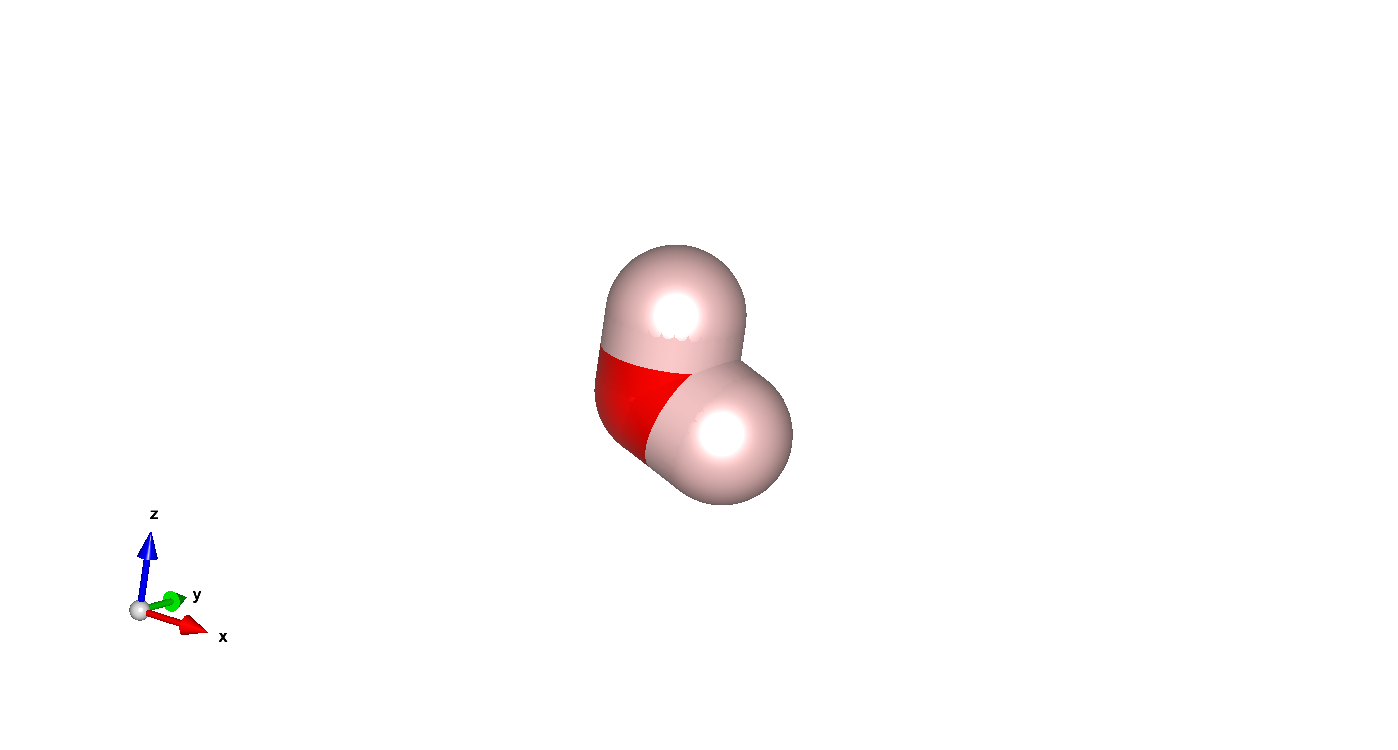
\includegraphics[width = \textwidth]{water.png}
		\caption{Molécule d'eau}
	\end{subfigure}
	\caption{Structures des molécules provenant de la COD}
	\label{fig:molecules_initiales}
\end{figure}

Puis, la structure de graphite de base a pu être étendue grâce à un logiciel tier\cite{momma_vesta_2011}, \num{9} fois selon la direction $[OX)$ et \num{5} fois selon la direction $[OY)$ afin que les dimensions dans ces directions soient du même ordre, pour obtenir une électrode de graphite (\autoref{tab:dimensions_structures} et \autoref{fig:electrode}).

\begin{table}[htb]
    \centering
    \begin{tabular}{l c c c}
        \hline
        Structure &X [Å] &Y [Å] &Z [Å]\\
        \hline
        Graphite de base &\num{2.456} &\num{4.254} &\num{6.696}\\
        Électrode de graphite &\num{22.104} &\num{21.270} &\num{6.696}\\
        \hline
    \end{tabular}
    \caption{Dimensions des sctructures}
    \label{tab:dimensions_structures}
\end{table}

\begin{figure}[htb]
    \centering
    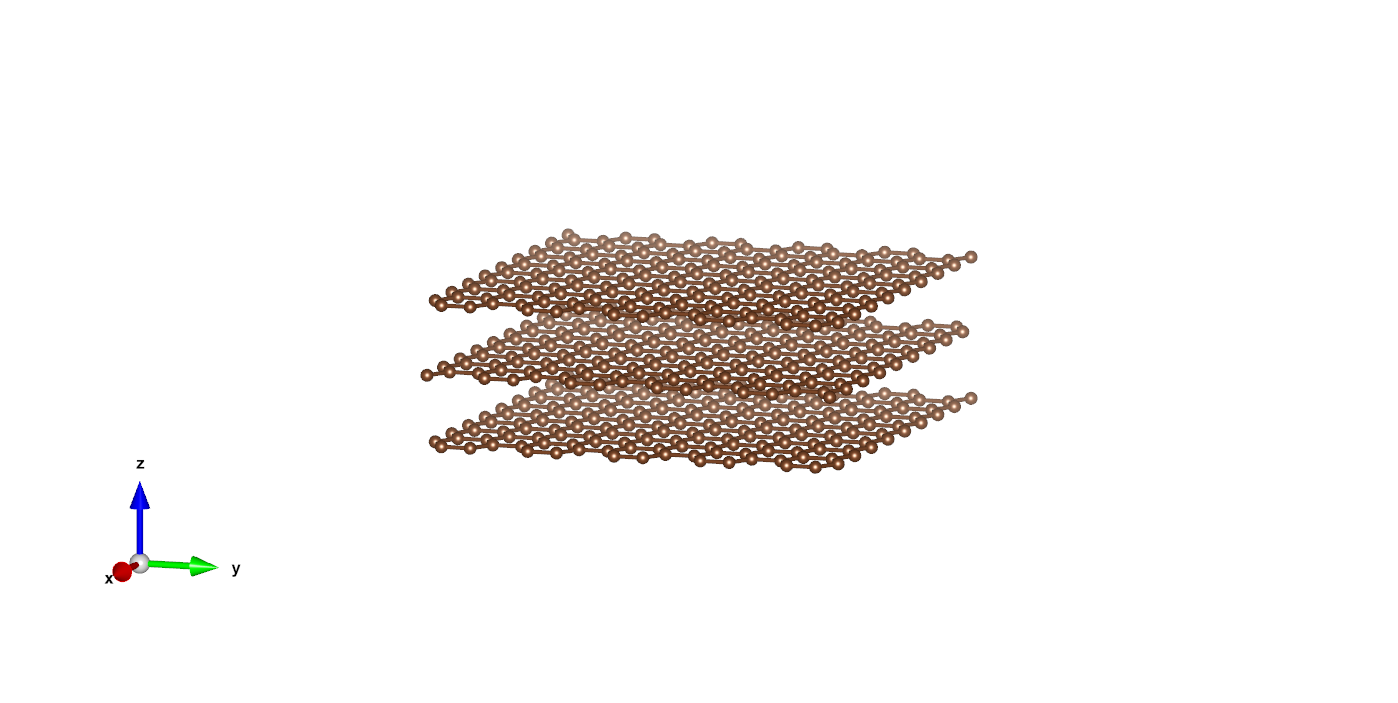
\includegraphics[width = \textwidth]{electrode.png}
    \caption{Électrode obtenue après duplication du réseau de graphite}
    \label{fig:electrode}
\end{figure}

Enfin, les molécules ont pu être disposées pour construire le modèle à l'aide de \emph{Packmol}\cite{martinez_packmol_2009}, \autoref{apdx:packmol}.\\
Pour obtenir des configurations initiales suffisamment stables nous avons choisi de répartir les entités en les séparant d'au moins \qty{2.5}{\angstrom} : entre les molécules et ions de l'électrolyte, et entre les particules de l'électrolyte et les électrodes.\\
Pour respecter les conditions aux limites périodiques, cette séparation a également été appliquée aux bords du système : nous ajoutons un retrait égal à la moitité de cette séparation à chaque bord.\\
Finalement, nous obtenons la configuration présentée à la figure \autoref{fig:structure_finale}.

\begin{figure}[hbp]
    \centering
    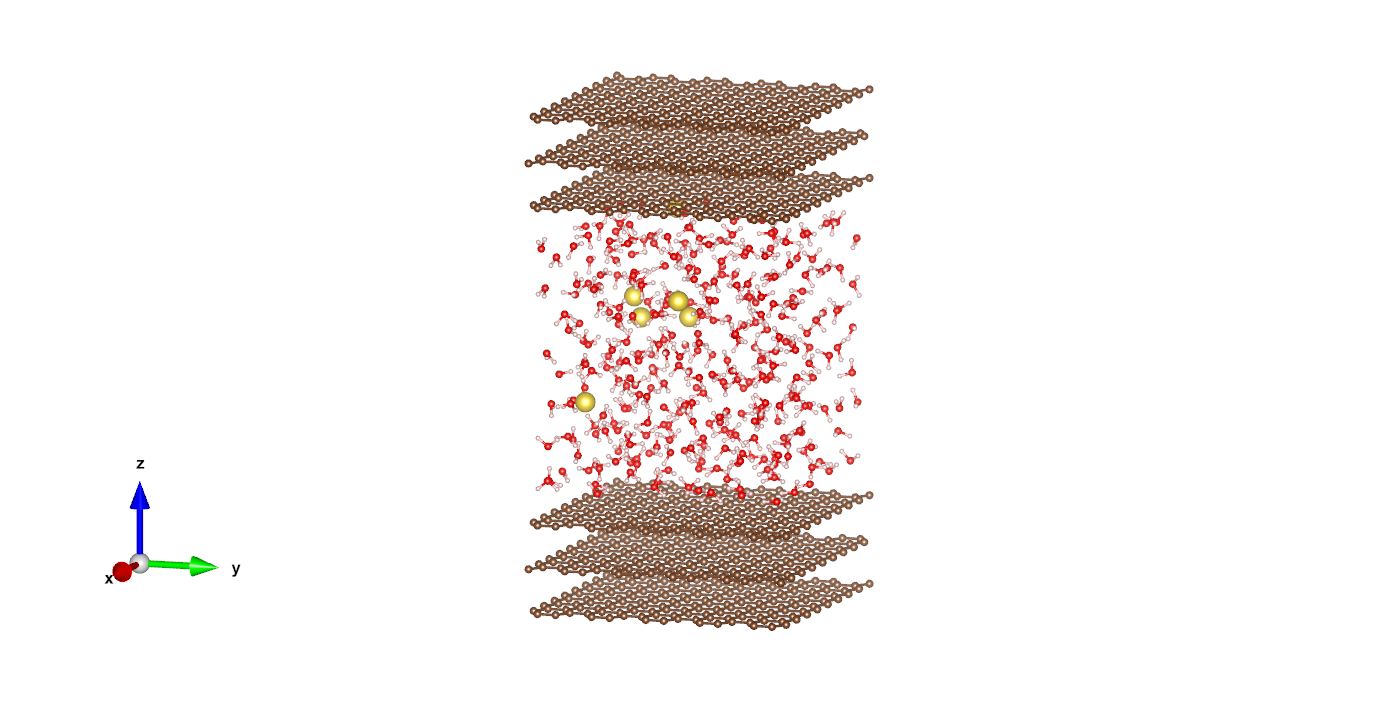
\includegraphics[width = \textwidth]{structure.png}
    \caption{Structure finale obtenue après agencement des molécules}
    \label{fig:structure_finale}
\end{figure}

% Simulations details
    \subsection{Déroulement et détails des simulations}

Pour toutes les simulations, le déroulement de la \autoref{fig:deroulement_simulations} a été adopté.

\begin{figure}[htp]
    \centering
    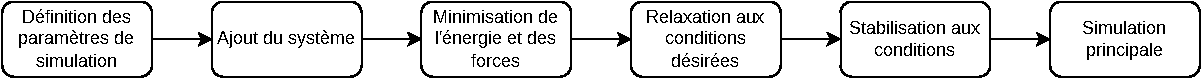
\includegraphics[width = \textwidth]{deroulement_simulations.pdf}
    \caption{Déroulement des simulations}
    \label{fig:deroulement_simulations}
\end{figure}

Pour la paramétrisation de la simulation :
\begin{itemize}
    \item les simulations ont un pas de temps (désigné \lstinline!timestep!) de \qty{0.1}{\femto \second} afin de prendre en compte les vibrations intramoléculaires (notamment celles de la molécule d'eau). 
    \item les interactions sont basés sur le potentiel réactif \emph{ReaxFF} dont nous discutons plus loin ().
    \item la polarisation du système, c'est-à-dire la mise en place de la différence de potentiel entre les électrodes, est réalisée grâce à \emph{EChemDID} que nous détaillons plus tard ().
\end{itemize}

Quant à l'ajout du système, ceci est effectué avec une commande \emph{LAMMPS} de lecture de données. Pour cela, il est nécessaire de convertir les données des positions des particules du système en données \emph{LAMMPS}, nous détaillons la démarche suivie à l'\autoref{apdx:conversion_lammps}.

Ensuite, la minimisation est réalisée par \emph{LAMMPS}, elle consiste à déplacer les particules du système sans dynamique de manière à minimiser l'énergie potentielle et les forces totales du système. Cette procédure suit un algorithme de gradient conjugué avec pour fonction objectif l'énergie potentielle totale :
\begin{equation}
    E(r_1, r_2, \dots, r_N) = \sum_{i, j} E_{pair} (r_i, r_j) + \dots + \sum_{i, j} E_{fix} (r_i)
\end{equation}
prenant en compte l'énergie des interactions de paires, des liaisons et angles si présents, des interactions \textit{improper} ou \textit{dihedral}, et des \lstinline!fix! imposés lors de la minimisation (ex : ajout de contraintes, de forces appliquées sur les atomes, etc.).

Puis, la relaxation et la stabilisation utilisent un thermostat et barostat de Nosé--Hoover -- c'est-à-dire dans l'ensemble canonique -- pour atteindre les conditions physiques recherchées puis les stabiliser. Les quantités thermodynamiques lors de ces étapes sont typiquement celles des \autoref{fig:allures_thermostat_barostat}.

\begin{figure}[htp]
    \centering
    \begin{subfigure}[t]{.49\textwidth}
        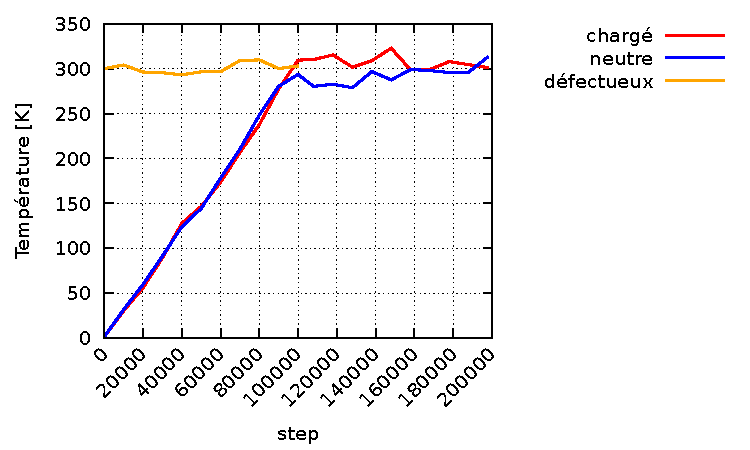
\includegraphics[width = \textwidth, draft]{relaxation_temp.pdf}
        \caption{Température}
    \end{subfigure}%
    ~
    \begin{subfigure}[t]{.49\textwidth}
        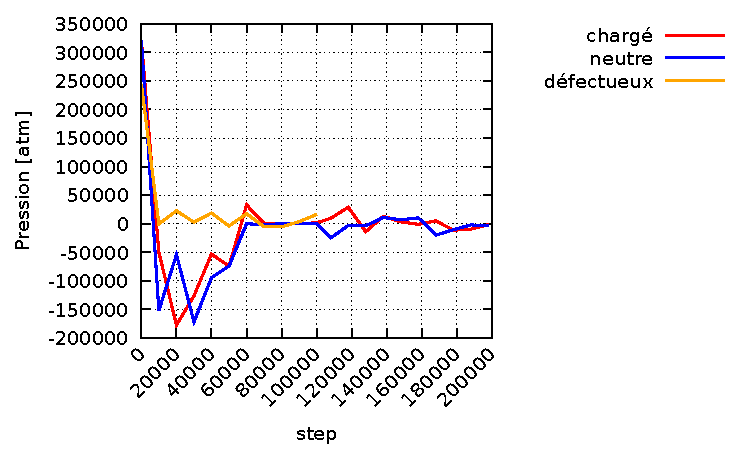
\includegraphics[width = \textwidth, draft]{relaxation_press.pdf}
        \caption{Pression}
    \end{subfigure}
    \begin{subfigure}[t]{.49\textwidth}
        \includegraphics[width = \textwidth, draft]{relaxation_density.pdf}
        \caption{Densité}
    \end{subfigure}
    \caption{Allures des grandeurs thermodynamiques pendant de la relaxation et la stabilisation {\tiny (chaque étape a lieu en \num{100000} \lstinline!timestep!s soit \qty{10}{\pico \second})}}
    \label{fig:allures_thermostat_barostat}
\end{figure}

Enfin, la simulation principale se déroule avec un thermostat du même type -- sans barostat cette fois -- et avec une durée plus longue ($\geq~\qty{1}{\nano \second}$) pour permettre l'équilibration du système (\autoref{fig:allures_simulation_principale}).

\begin{figure}[hbp]
    \centering
    \begin{subfigure}[t]{.49\textwidth}
        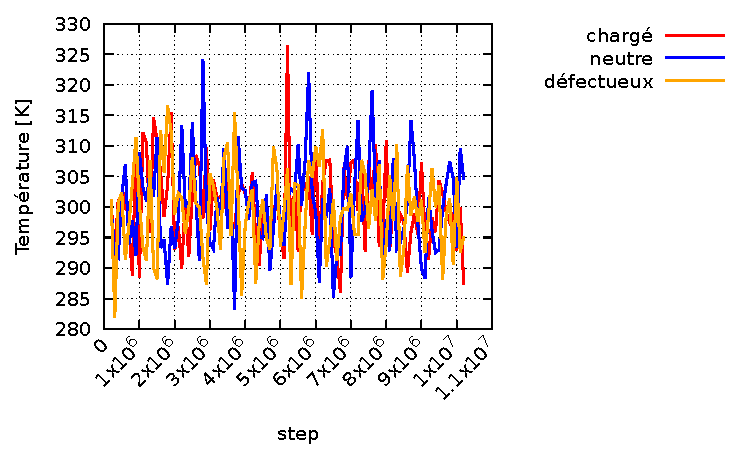
\includegraphics[width = \textwidth, draft]{main_temp.pdf}
        \caption{Température}
    \end{subfigure}%
    ~
    \begin{subfigure}[t]{.49\textwidth}
        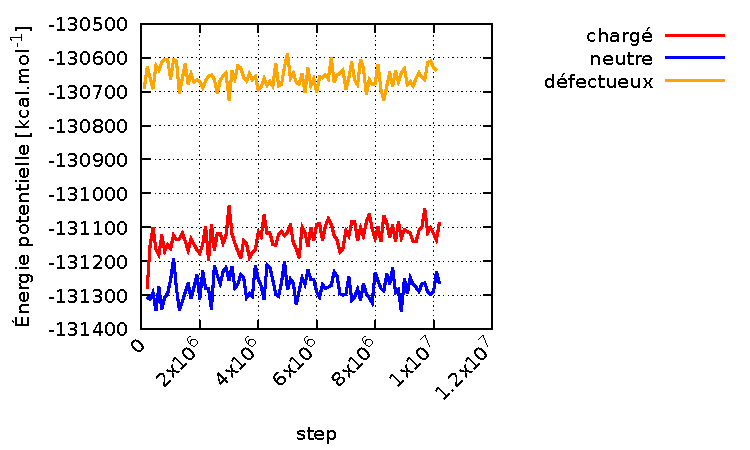
\includegraphics[width = \textwidth, draft]{main_epot.pdf}
        \caption{Énergie potentielle}
    \end{subfigure}
    \begin{subfigure}[t]{.49\textwidth}
        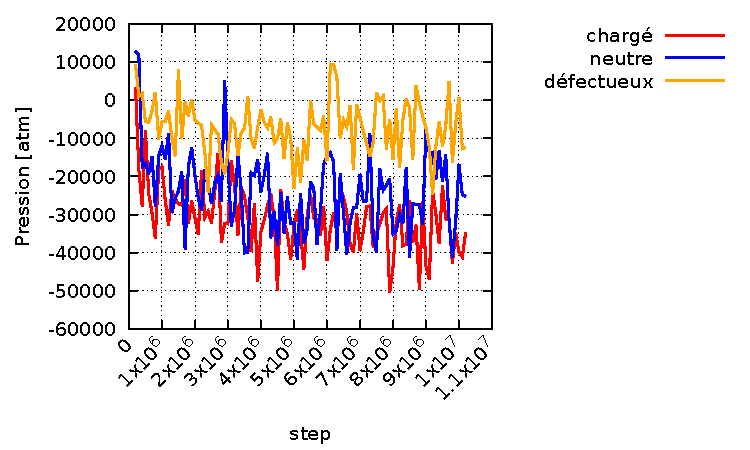
\includegraphics[width = \textwidth, draft]{main_press.pdf}
        \caption{Pression}
    \end{subfigure}
    \caption{Allures des grandeurs thermodynamiques pendant la simulation principale}
    \label{fig:allures_simulation_principale}
\end{figure}
